\chapter{Part E: Implied volatility surface}
Developer: Joseph Perez

\noindent Validator: Simon Leger

%DEVELOPER WRITES THIS PART --->

\section{Requirements}

Giving a matrix of call and put prices for a range of maturities and strikes and a yield curve allows us to invert the Black-Scholes formula for each price to get the implied volatility.
In plotting the matrix of implied volatilites we create an implied volatility surface.

According to Black-Scholes option pricing model, the volatility for calls and puts for the same maturity should have the same volatility of the stock price and the implied volatility surface should be a term structure.
However market prices indicate that volatilities depend on strikes level.
The implied volatility surface of market prices looks like a smile.

\section{Design }

We build an implied volatility surface for an underlying from its price, a yield curve and a table of standard european call/put prices for different maturities and different strikes.

Black-Scholes' model makes it possible to price a call or a put with closed form solution if we consider constant volatility  and constant interest rate. But the classical option pricing formulas can be inverted and we can compute what is commonly call the implied volatility if we know the price.

According to Black-Scholes option pricing model, the volatility for calls and puts for the same maturity should have the same volatility of the stock price and the implied volatility surface should be a term structure.
However market prices indicate that volatilities depend on strikes level.
The implied volatility surface shape can be different depending on the underlying. Smile, smirk or sneer are kinds of name we give to caracterize those shapes. For equity index options markets, it is more of a skewed curve. This has motivated the name  "volatility skew".




European options on stock are often liquid and option prices are given by the market. We use for the price the midpoint of Bid/Ask.



\section{Approach}
%<high-level description of the design>

\section{Choices}
Once our price inverted we have a range of implied volatilites for different levels of strike and different maturities. Then we can get the implied volatity (or variance) for a given strike and a given maturity using a quadratic interpolation.
As the implied volatility surface is rather smooth a local 2D quadratic interpolation gives us good approximation.


\section{Methods}
For each maturity and each strike for which we have the price of a call or a put, we create a BlackScholes object. The constructor of BlackScholes class inverts Black-Scholes formula using the recursive Newton-Raphson algorithm in order to get the implied volatility.

Once the implied volatility surface is set we can compute the implied volatility (or variance) for any maturity and any strike.
To do this we use the 2D-quadratic interpolator.
As the surface is rather smooth and looks like a parabol, a quadratic interpolation gives us good approximation.

The class includs a method to compute a forward volatility. Assuming we built our implied volatility surface at time $t$ and we want to know what would look like the volatility at time $T_2$ seen at $T_1$ for a strike $K$. We use the following formula
\[
\sigma_{T_1,T_2}^2(K)=\frac{\sigma_{T_2}^2(K)(T_2-t)-\sigma_{T_1}^2(K)(T_1-t)}{T_2-T_1}
\]
%<brief descriptions of methods - can take from doxygen documentation>

\section{Unit tests}
We build the implied volatility surface for the S$\&$P500 from call and put prices of July 2004. The shape we get is as expected, it is a "skewed surface".
\begin{figure}
\begin{center}
        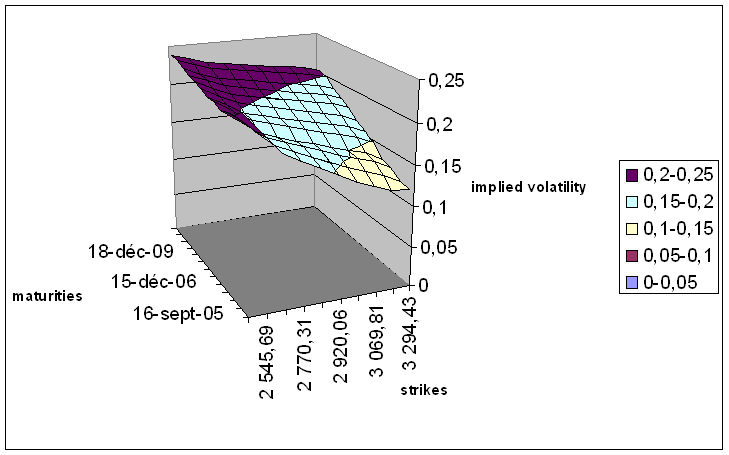
\includegraphics[width=12cm]{volsurfjoseph.jpg}
        \caption{Volatility surface of S$\&$P500}
\end{center}
\end{figure}

\section{Performance}

The Vega of call/put is always positive option prices are increasing function of the volatility that's why Newton-Raphson algorithm is accurate in this case. By default inversion of Blacks Scholes formula return the computed volatility after 100 iterations. In practice the volatility converges quickly, only 10 iterations are necessary. So we could either set the number of iterations to be 20 or to compare after each iteration the difference $|\s_{n+1}-\s_n|$ and exit the loop as it is inferior to a level $\epsilon$.

%VALIDATOR WRITES THIS PART --->

\section{Validation}


\subsection{Approach}

%<i.e. what alternate method was used to validate the results - if this required a lot of code then similar outline as above should apply>

To test this class, whose accuracy is very important for the rest of the project, we ran two tests. 
First we instanciated an object of the volsurface using the flat volatility constructor and we 
checked that every point was giving the same and correct volatility and we also checked the 
values of forward volatilities in an Excel spreadsheet by replicating the formula. 
\par Then we created a bench of strikes and dates in an Excel spreadsheet and by choosing a volatility 
for these points, just arbitrary. We compute the black scholes price for each of these options 
and we load these prices, dates and strikes into our c++ project and construct the yieldcurve with them. 
After this, we decide to get some volatility from this object for some strikes and matuirties and we check 
if they give exactly the same result than for the inputs and nice enough results for other points.
Then we simply plot the volatility surface in a two dimensional chart to check its shape.
\par Here is the table for these volatilities given the strikes and maturities transformed in years :

\noindent
\begin{tabular}{rrrrrrrrrrr}

  maturity &    2395.95 &    2545.69 &    2695.44 &    2770.31 &    2845.19 &    2920.06 &    2994.93 &    3069.81 &    3144.68 &    3294.43 \\

 0.1697467 &        0.2 &       0.19 &       0.18 &       0.17 &       0.16 &       0.15 &       0.14 &       0.13 &       0.12 &       0.11 \\

 0.6680356 &       0.22 &       0.21 &        0.2 &       0.19 &       0.18 &       0.17 &       0.16 &       0.15 &       0.14 &       0.13 \\

 1.4154689 &       0.24 &       0.23 &       0.22 &       0.21 &        0.2 &       0.19 &       0.18 &       0.17 &       0.16 &       0.15 \\

 2.4312115 &       0.26 &       0.25 &       0.24 &       0.23 &       0.22 &       0.21 &        0.2 &       0.19 &       0.18 &       0.17 \\

 4.4243669 &       0.28 &       0.27 &       0.26 &       0.25 &       0.24 &       0.23 &       0.22 &       0.21 &        0.2 &       0.19 \\

 7.4332649 &        0.3 &       0.29 &       0.28 &       0.27 &       0.26 &       0.25 &       0.24 &       0.23 &       0.22 &       0.21 \\

\end{tabular}  
As one can see we constructed a linear volsurface, increasing with maturity and decreasing with strike, and here is the plot of this surface :

\begin{figure}
\begin{center}
        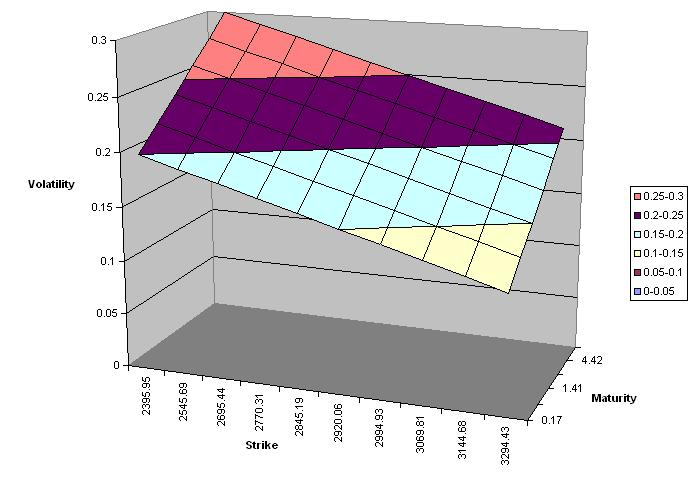
\includegraphics[width=12cm]{volsurf1.jpg}
        \caption{Linear Volatility surface}
\end{center}
\end{figure}

